
\documentclass[../../main.tex]{subfiles}
\graphicspath{{\subfix{../../images/}}}

\begin{document}

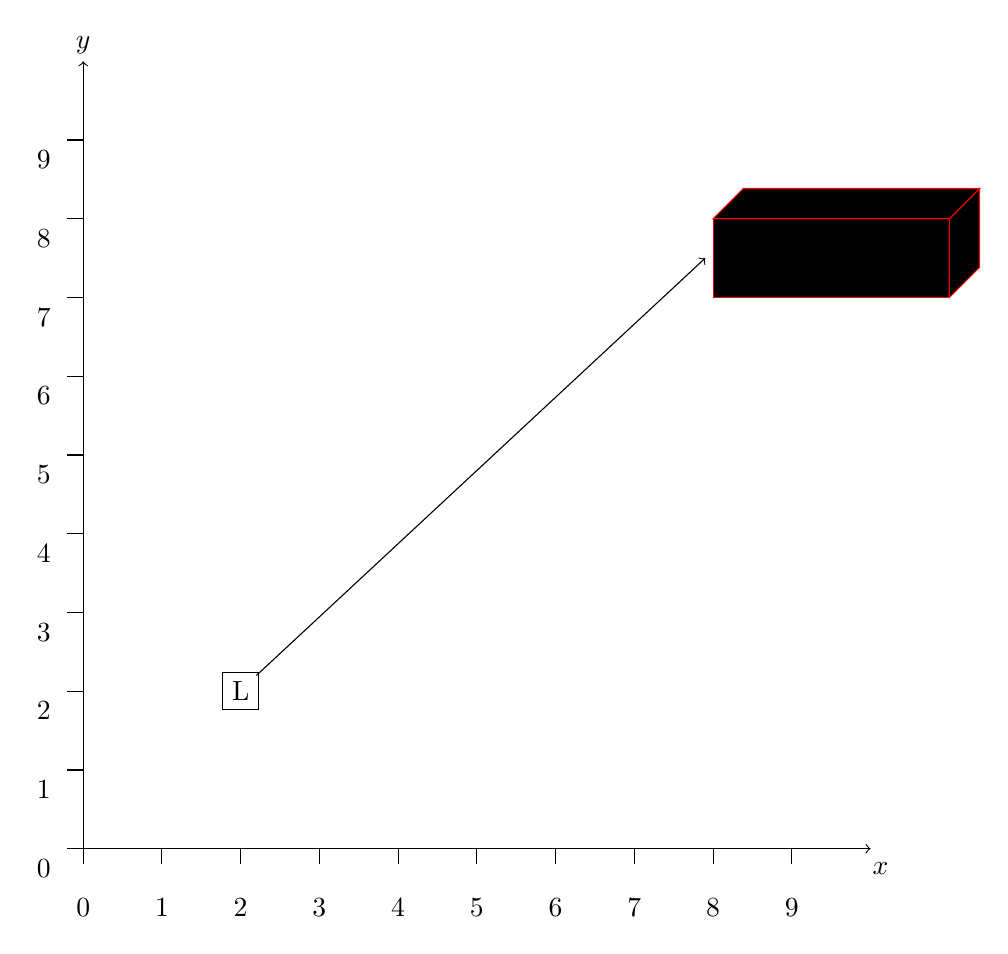
\begin{tikzpicture}
\draw[->] (0, 0) -- (0, 10);
\draw[->] (0, 0) -- (10, 0);
\node at (0, 10.2) {$y$};
\node at (10.125, -0.25) {$x$};
\foreach \x in {0, 1, 2, 3, 4, 5, 6, 7, 8, 9}
{
\draw (\x,0) -- (\x,-0.2);
\node at (\x,-0.75) {$\x$};
\draw (0, \x) -- (-0.2, \x);
\node at (-0.5, \x-0.25) {$\x$};
}
\coordinate (m) at (2,2);
\draw[->] (2.2, 2.2) -- (7.9, 7.5);

\pgfmathsetmacro{\cubex}{3}
\pgfmathsetmacro{\cubey}{1}
\pgfmathsetmacro{\cubez}{1}
\draw[red,fill=black] (11,8,0) -- ++(-\cubex,0,0) -- ++(0,-\cubey,0) -- ++(\cubex,0,0) -- cycle;
\draw[red,fill=black] (11,8,0) -- ++(0,0,-\cubez) -- ++(0,-\cubey,0) -- ++(0,0,\cubez) -- cycle;
\draw[red,fill=black] (11,8,0) -- ++(-\cubex,0,0) -- ++(0,0,-\cubez) -- ++(\cubex,0,0) -- cycle;


\node[draw,align=left] at (2, 2) {L};

\end{tikzpicture}
\\\\Das weiße Licht scheint von L(2, 2, 2) auf die Normale N(8, 8, 0) eines Schokoriegels. \\Der Schokoriegel hat am Punkt der Normalen den $RGB_D$-Wert (0.01, 0.01, 0.01). 
\\\\
Berechne die Farbe der diffusen Beleuchtungskomponente.

\end{document}


